\subsubsection{usergoal-ugAdministrateTheSystem}

\label{RE-use-case-ugAdministrateTheSystem}



the actAdministrator's goal is to follow an identification procedure to be allowed to add or delete the necessary crisis coordinators that will be granted the responsibility to handle alerts and crisis. 


\begin{usecase}
  \addheading{Use-Case Description}
  \addsingletwocolumnrow{Name}{ugAdministrateTheSystem}
  \addsingletwocolumnrow{Scope}{system}
  \addsingletwocolumnrow{Level}{usergoal}
  

\addrowheading{Primary actor(s)}
\addnumberedsinglerow{}{\msrcode{actAdministrator[active]}}



\addrowheading{Goal(s) description}
\addsinglerow{
the actAdministrator's goal is to follow an identification procedure to be allowed to add or delete the necessary crisis coordinators that will be granted the responsibility to handle alerts and crisis. 
}

\addrowheading{Reuse}
\addnumberedsinglerow{}{\msrucname{ugSecurelyUseSystem [1..*]}}
\addnumberedsinglerow{}{\msrucname{oeAddCoordinator [1..*]}}
\addnumberedsinglerow{}{\msrucname{oeDeleteCoordinator [0..*]}}

\addrowheading{Protocol condition(s)}
\addnumberedsinglerow{}{
the iCrash system has been deployed
}

\addrowheading{Pre-condition(s)}
\addnumberedsinglerow{}{
none
}

\addrowheading{Main post-condition(s)}
\addnumberedsinglerow{}{
modifications have been made to the system and its environment concerning existing or new coordinators.
}

\addrowheading{Main Steps}
\addalphanumberedsinglerow{}{the actor \msrcode{actAdministrator} executes the \msrucname{ugSecurelyUseSystem} use case}
\addalphanumberedsinglerow{}{the actor \msrcode{actAdministrator} executes the \msrucname{oeAddCoordinator} use case}
\addalphanumberedsinglerow{}{the actor \msrcode{actAdministrator} executes the \msrucname{oeDeleteCoordinator} use case}
\addrowheading{Steps Ordering Constraints}
\addnumberedsinglerow{}{steps (a) (b) and (c) executions are interleaved 
          (steps (b) and (c) have their protocol constrained 
           by steps of (a)).}
\addnumberedsinglerow{}{steps (a) (b) and (c) can be executed multiple times.}


\end{usecase} 


Figure \ref{fig:ru.iu.bachelor.sed.group01.icrash-RE-UCD-uc-ugAdministrateTheSystem}
shows the use case diagram for the ugAdministrateTheSystem user goal use case

\begin{figure}[htbp]
\begin{center}

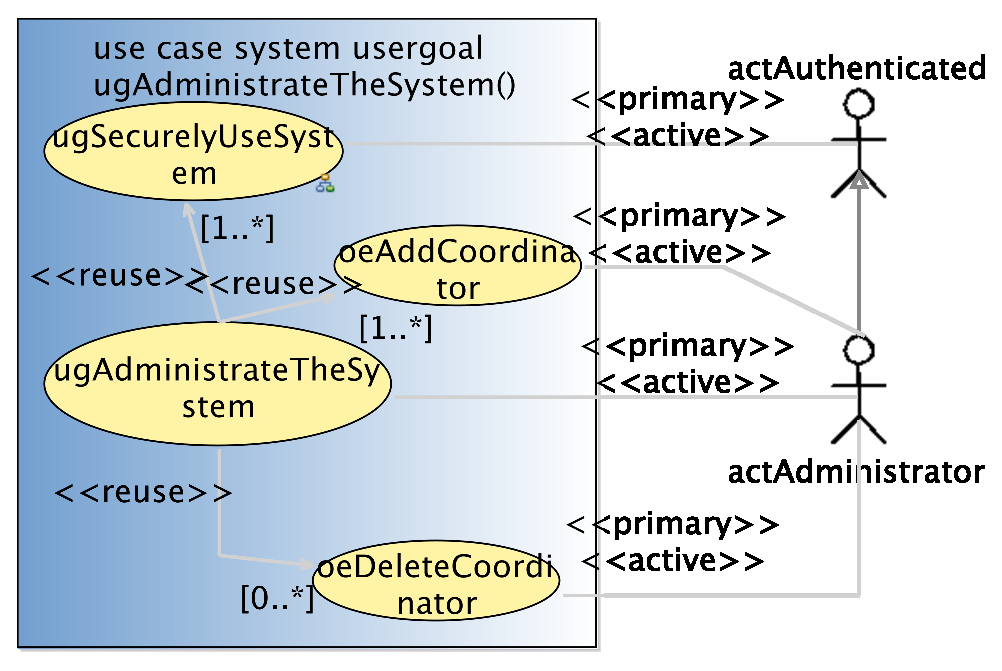
\includegraphics[
angle=0
,scale=0.75
]{./images-report-gen/usecase-model/usergoal/uc-ugAdministrateTheSystem.eps}
\end{center}
\caption[ru.iu.bachelor.sed.group01.icrash Use Case Diagram: uc-ugAdministrateTheSystem]{ ugAdministrateTheSystem user goal use case}
\label{fig:ru.iu.bachelor.sed.group01.icrash-RE-UCD-uc-ugAdministrateTheSystem}
\end{figure}
\vspace{0.5cm}
